\section{实验}

本章节将介绍本次实验的具体细节,包括实验环境、数据集、评价指标、实验结果等。之后将展示实验结果并进行分析,包括全局与局部特征分析、可视化分析、性能与泛化能力对比等。最后本章节将进行总结。

\subsection{实现细节}

% 硬件?环境?框架?超参数设置?
本文的实验代码使用Python语言编写,选用ConvNeXt-Base和ViT-16/B两种模型进行对比,两种模型同样在ImageNet-21K上进行预训练,选用224x224的图像分辨率。此外,两种模型具备相似的参数量,前者为89M,后者为87M。本文的所有实验在一台拥有4块NVIDIA V100 GPU的服务器上进行,实验使用PyTorch框架进行实现。

\subsection{数据集与评价指标}

本文用于降维可视化的主要数据集有CIFAR-10和CUB200两个数据集。CIFAR-10数据集包含10个不同的类别,如汽车、鸟类和猫等,这些类别之间的差异较大。CUB200数据集专注于鸟类图像,包含200个子类别,这些子类别间的差异相对较小,主要体现在鸟的种类、羽毛颜色和姿态等细微特征上。这两个数据集的选择旨在考察模型在不同数据集上的性能差异,以及对于不同类别之间的差异性的处理能力。

本文选择ImageNet-X和PUG-Imagenet两种数据集对模型的影响因素进行评估。ImageNet-X 数据集是一个用于探索模型错误影响因素,数据集提供了关于 16 种变化因素的详细人机注释,例如姿态、风格等。这使得可以有针对性地分析模型的错误类型。而PUG-ImageNet数据集是一个合成数据集,该数据集中的图像使用软件引擎生成,允许系统地改变每个对象的姿势、大小、纹理、光线和
背景等因素,从而通过控制这些因素来评估模型的性能。

为了探究模型的跨域泛化能力,本文选择ImageNet-Sktech、ImageNet-V2、ImageNet-R、ImageNet-A 4种数据集,这些数据集都是ImageNet数据集的变种,用于评估模型在不同数据集上的泛化能力。ImageNet-Sktech数据集是一个手绘图像数据集,ImageNet-V2数据集是一个用于评估模型在真实世界中的泛化能力的数据集,ImageNet-R数据集是一个用于评估模型在不同分辨率下的泛化能力的数据集,ImageNet-A数据集是一个用于评估模型在不同摄像机角度下的泛化能力的数据集。此外,为了探究模型的跨数据集泛化能力,本文选择Pets、Caltech101、CIFAR-100、DTD、Flowers102、SUN397、EuroSAT 7种数据集,这些数据集拥有不同的类别,如动物、植物、环境、纹理、卫星图像等,用于评估模型在不同数据集上的泛化能力。

本文的主要评价指标有轮廓系数、域内准确率和域外准确率等,这些指标用于评估模型在不同数据集上的性能差异。轮廓系数是一个衡量聚类质量的指标,其值越接近于1,说明聚类内的相似度高而聚类间的差异大,聚类效果越好。域内准确率和域外准确率分别用于评估模型性能,模型通过在域内、域外数据集上进行微调之后进行测试得到准确率,通过比较模型在域内、域外数据集上的准确率,可以评估模型的泛化能力。

\subsection{实验结果}

\subsubsection{全局和局部特征分析}

\begin{figure}[H]
    \centering
    \subfigure[ViT]{
        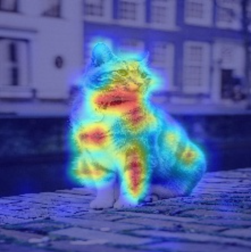
\includegraphics[width=0.33\textwidth]{pics/cat_grad.png}
    }
    \subfigure[ConvNeXt]{
        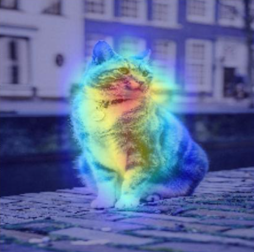
\includegraphics[width=0.33\textwidth]{pics/cat_grad1.png}
    }
    \\
     \caption{ViT和ConvNeXt的Grad-CAM可视化注意力图}
    \label{fig:grad}
\end{figure}

通过分别选取ViT模型和ConvNeXt模型的图像编码器的最后一层,进行梯度计算,得到图\ref{fig:grad}的结果。在图中可以较为明显的看到,两种模型在进行图像类时都能将注意力放在前景物体上,ViT的关注区间比较发散,而ConvNeXt比较集中,呈现从关注中心向四周散开的高斯形状。

这种观察表明ViT和ConvNeXt在处理图像时可能存在不同的注意力分布模式。ViT显示出的较为发散的关注区间可能反映了其自注意力机制的特性,该机制允许模型在图像的不同区域之间建立长距离的依赖关系。因此,ViT在处理图像时可能能够建立全局的信息,从而导致关注区间相对发散。相比之下,ConvNeXt呈现出的关注区间更加集中,呈现出从猫头为中心的高斯形状。这可能反映了传统卷积神经网络的特点,即它们会受到归纳偏置的影响。在处理图像时可能更加注重临近范围特定目标的捕捉,因此其关注区间更加集中于目标的中心区域。从上述表现中可初步说明ViT模型的注意力范围更远。

\begin{figure}[H]
    \centering
    \subfigure[ViT]{
        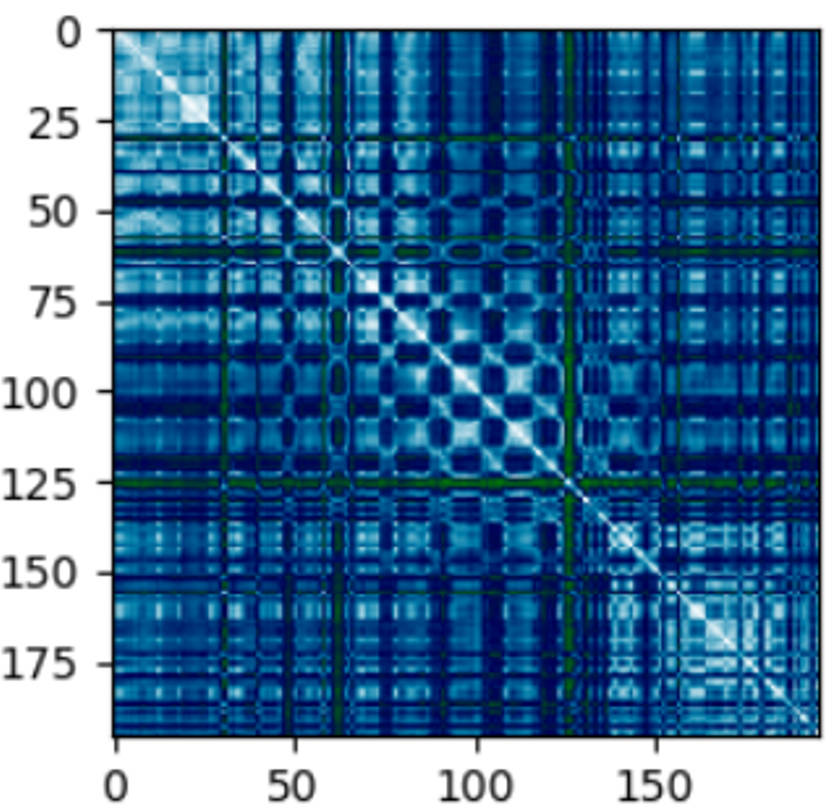
\includegraphics[width=0.4\textwidth]{pics/patch-smi2.jpg}
    }
    \subfigure[ConvNeXt]{
        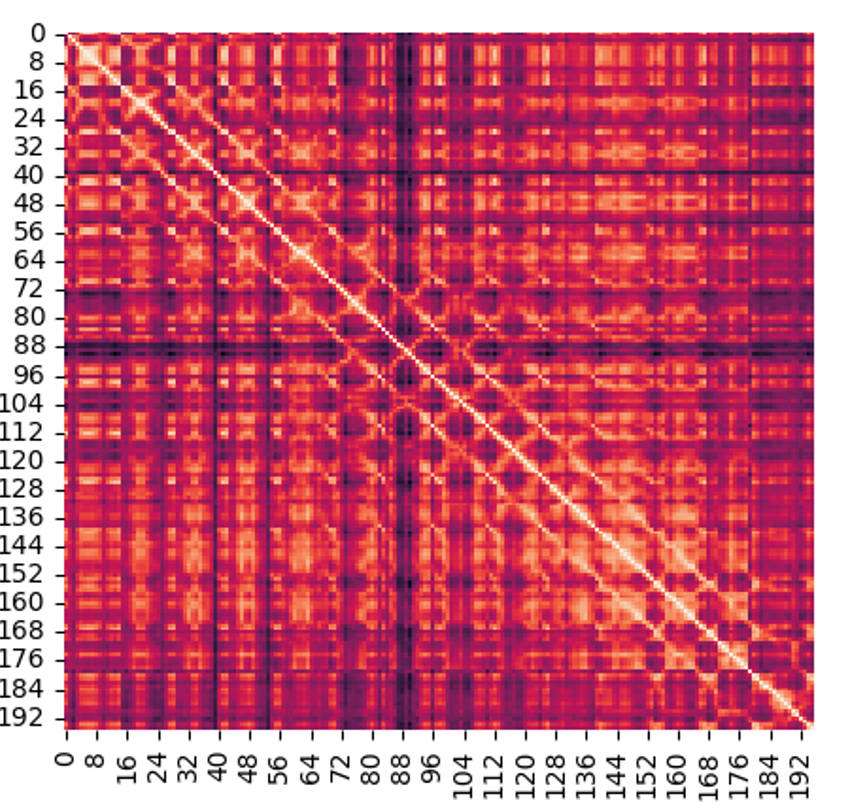
\includegraphics[width=0.4\textwidth]{pics/patch-smi.jpg}
    }
    \\
     \caption{ViT和ConvNeXt局部特征之间的相似度}
    \label{fig:patch-smi}
\end{figure}

为了进一步验证上述采样,本文对两个网络的局部相似度进行可视化分析。通过计算模型局部特征块两两之间的余弦相似度,得到图\ref{fig:patch-smi}的结果。如图所示,ConvNeXt的局部相似度矩阵中呈现出多条颜色较亮的斜平行线,这说明其中的每个局部块特征都与上下左右的相邻局部块特征之间存在更大的相似性。相比之下,ViT模型的局部块之间并没有存在明显的空间关系限制。这说明ConvNeXt更关注空间相似性,即空间关系会影响图像表征;ViT能够在全局范围内捕捉图像的长距离依赖关系,不受到像素之间空间关系的影响。这也说明了ConvNeXt形成类似高斯形状的注意力图,而ViT更为发散的原因。

\begin{figure}[H]
    \centering
    \subfigure[ViT]{
        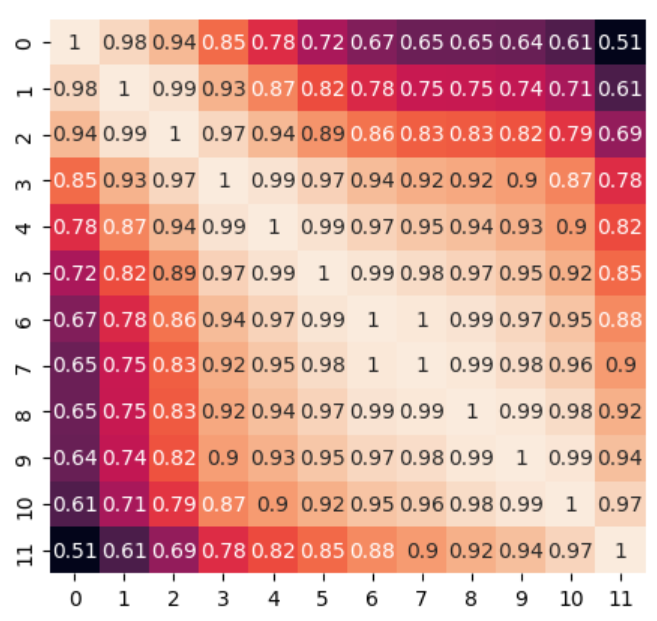
\includegraphics[width=0.4\textwidth]{pics/layer-smi.png}
    }
    \subfigure[ConvNeXt]{
        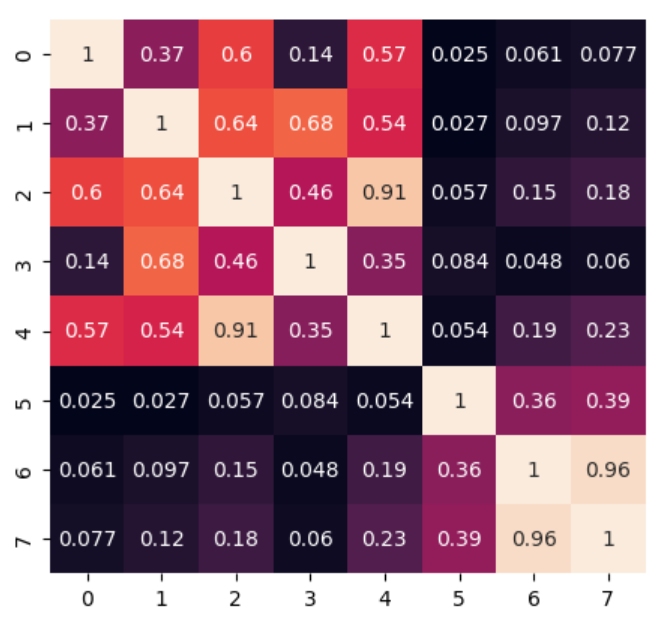
\includegraphics[width=0.4\textwidth]{pics/layer-smi1.png}
    }
    \\
     \caption{ViT和ConvNeXt层之间的CKA相似度}
    \label{fig:layer-smi}
\end{figure}

为了对比ConvNeXt和ViT模型在特征理解能力上的区别,本文提取模型逐层的特征进行分析。ViT注意力层输出特征,ConvNeXt使用卷积层输出特征。本文通过CKA方法分别计算两种模型每层结构的特征相似度,CKA方法可以有效度量不同维度向量之间的相似度,从而应对层之间的维度变化。得到层级之间的CKA相似度矩阵如图\ref{fig:layer-smi},从图中可看出,ViT模型在浅层时特征和高层时特征已有比较明显的相似性,说明其能在浅层时就学到比较高级的语义信息;相比而言,ConvNeXt模型的浅层和深层特征之间的相似度具有较大的区别,说明CNN需要逐层卷积才能逐渐聚合高层语义特征。

从归纳偏置的视角来看,ViT由于不受任何约束,浅层模块就可以学习长程注意力,提取全局特征。然而,在CNN的卷积操作中,每个区域只能与周围区域进行局部交互,这限制了浅层模块的全局特征提取能力,只能学习纹理、形状等低级语义信息。直到深层卷积聚合了浅层的局部信息之后,才能学习高级语义信息。这种机制更类似于人类大脑的工作机制,首先提取局部信息,之后聚合全局信息。

\begin{figure}[H]
    \centering
    \subfigure[ViT]{
        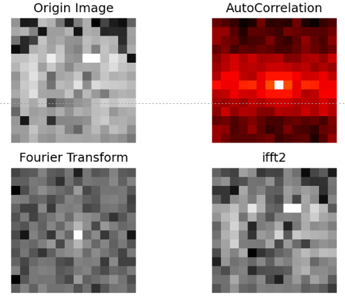
\includegraphics[width=0.4\textwidth]{pics/fft1.png}
    }
    \subfigure[ConvNeXt]{
        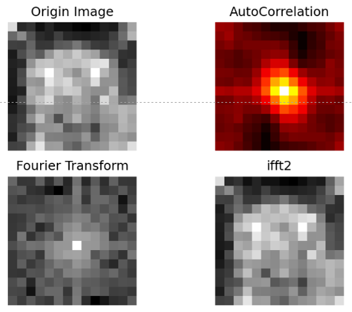
\includegraphics[width=0.4\textwidth]{pics/fft2.png}
    }
    \\
     \caption{ViT和ConvNeXt的频域分析}
    \label{fig:fft}
\end{figure}

\begin{figure}[H]
    \centering
    \subfigure[ViT特征图]{
        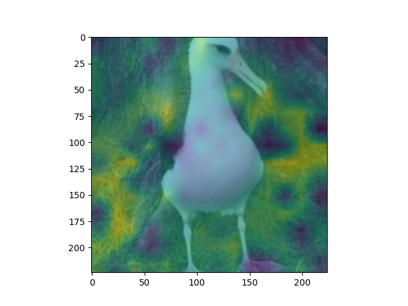
\includegraphics[width=0.45\textwidth]{pics/feat_mmap.png}
    }
    \subfigure[ConvNeXt特征图]{
        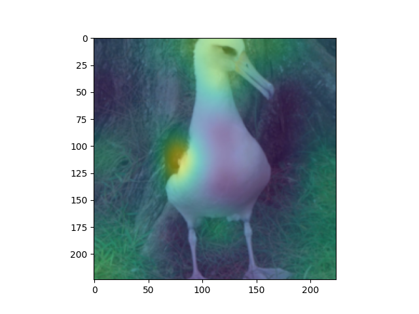
\includegraphics[width=0.45\textwidth]{pics/feat_map2.png}
    }
    \\
     \caption{ViT和ConvNeXt特征图可视化}
    \label{fig:feat_map}
\end{figure}

为了进一步说明ViT模型与ConvNeXt在学习能力上差异,本文对特征进行频域分析。如图
\ref{fig:fft}所示,ViT的低频和高频信息都受到高度激活,这说明ViT能够兼顾低频和高频信息。另外,ConvNeXt的低频信息激活明显,而高频信息激活并不明显,这说明CNN倾向于学习低频信息。通过频域分析,本文发现ViT比CNN更倾向于细节信息,这也可能导致模型在噪声上容易过拟合。

图\ref{fig:feat_map}展示了ViT的一种过拟合情形,通过对特征在通道上求均值,得到模型的感兴趣区域。从图中可以看出,ViT倾向于关注图像中的背景噪声,而ConvNeXt是比较精准的关注在了前景物体的关键部位。这可能是由于CNN模型的归纳偏置限制了感兴趣区域的形状,使得模型倾向于关注到与任务相关的主要特征。而ViT缺乏这种限制,使得模型发散到无关特征上。因此,CNN的归纳偏置能够在一定程度上能够减轻无关背景细节的影响,减轻过拟合现象。

\subsubsection{降维特征分析}

在使用t-SNE进行降维分析的过程中,在图\ref{fig:tsne}的子图(a)(b)可以清楚地看到CIFAR-10和CUB200两个数据集中不同模型的表现差异。对于通用数据集CIFAR-10来说,两种模型都有不错的特征分布;然而对于细粒度数据集CUB200来说,ConvNeXt的特征分布要比ViT更优。

\begin{figure}[H]
    \centering
    \subfigure[ConvNeXt在cifar10上的特征可视化]{
        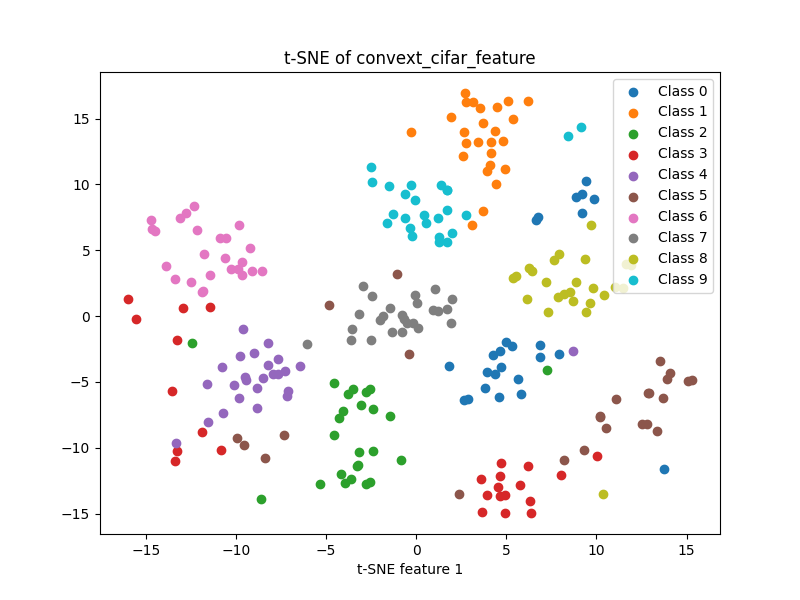
\includegraphics[width=0.45\textwidth]{pics/t-SNE of convext_cifar_feature_25.png}
    }
    \subfigure[ViT在cifar10上提取到的特征可视化]{
        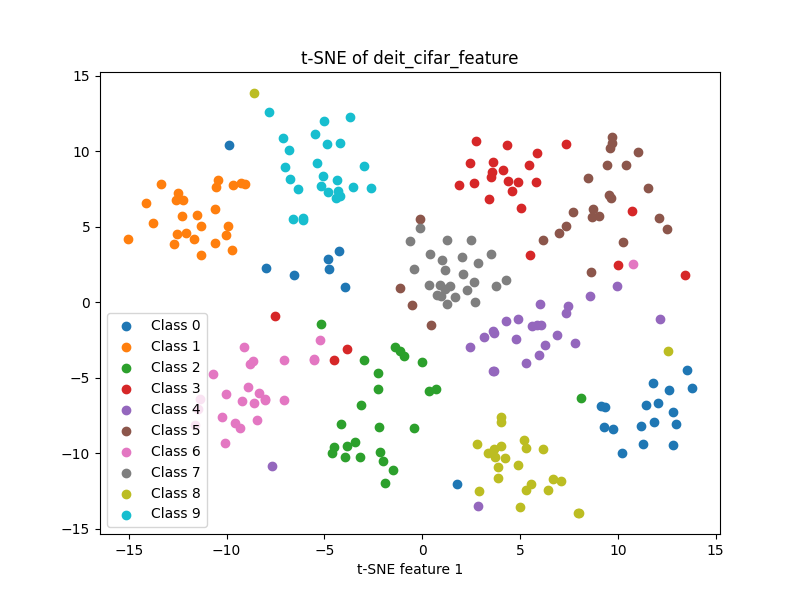
\includegraphics[width=0.45\textwidth]{pics/t-SNE of deit_cifar_feature_25.png}
    }
    \\
    \subfigure[ConvNeXt在CUB200上的特征可视化]{
        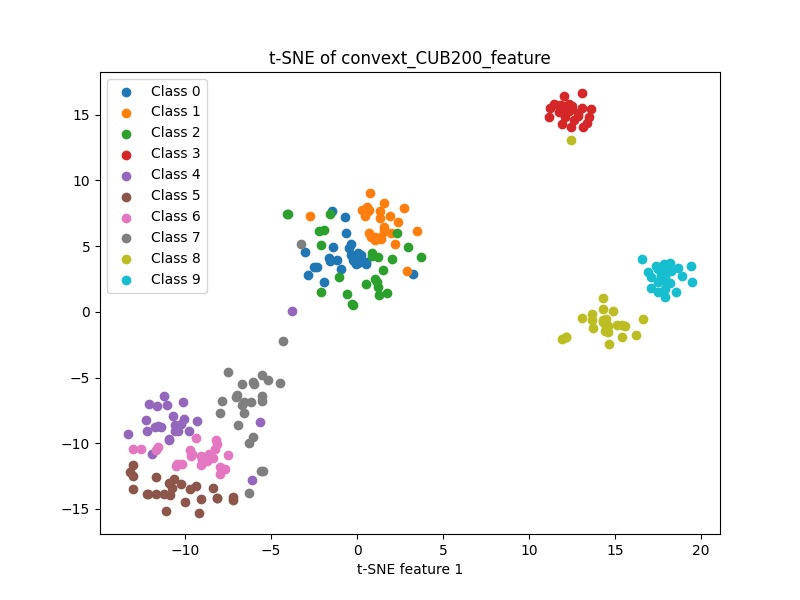
\includegraphics[width=0.45\textwidth]{pics/t-SNE of convext_CUB200_feature_25.png}
    }
    \subfigure[ViT在CUB200上的特征可视化]{
        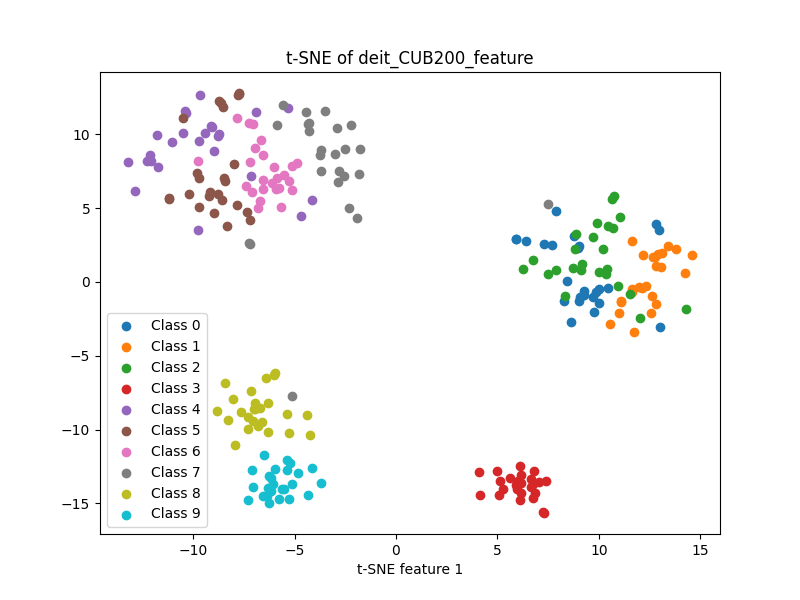
\includegraphics[width=0.45\textwidth]{pics/t-SNE of deit_CUB200_feature_25.png}
    }
    \caption{ViT和ConvNeXt在CUB200和cifar10上的特征可视化}
    \label{fig:tsne}
\end{figure}

为了量化特征分布的优劣程度,本文通过计算轮廓系数,进一步验证了这些观察结果。表\ref{tab:Silhouette Coefficient}反映了两种模型的轮廓系数。从表中可以看出,在CIFAR-10中ConvNeXt的轮廓系数和ViT接近,表现都非常好。在CUB200数据集上,ConvNeXt的轮廓系数明显高于ViT。这强调了ConvNeXt在处理包含细微局部差异的数据集时的优势,尤其是在CUB200这样的高度专业化的数据集上。ConvNeXt的高性能主要归因于其优秀的局部特征提取能力,这使得它在相似类别之间也能够有效地区分。

\begin{table}[H]
    \tabcolsep=40pt
    \centering
    \caption{ViT和ConvNeXt在两种数据集上的轮廓系数}
    \label{tab:Silhouette Coefficient}
    \begin{tabular}{c|cc}
          \hline
         &ViT  & ConvNeXt  \\
         \hline
         CUB200 &  0.113 & 0.130   \\
         CIFAR10 & 0.117 & 0.124 \\
         \hline
    \end{tabular}
\end{table}

\subsubsection{性能与泛化能力对比}

要想分析图像分类错误的影响因素,仅仅识别出错误的物体类别远远不够,关键在于找出这些错误的具体原因。例如,某些模型可能对数据分布的某些方面特别敏感,比如纹理变化。在这种情况下,当物体的纹理与它所训练的数据不同的时候,模型可能会一直出错。识别错误类型可以让有针对性地收集和重新训练数据,比黑盒方法具有优势。ImageNet-X数据集提供了关于16种变化因素的详细人机注释,例如姿态、风格等。本文选用该数据集,通过控制变量对影响因素进行分析,从而有针对性地分析模型的错误类型。

为了分析每种因素对模型错误率等影响,本文提出如下指标进行评估:

\begin{equation}
    \label{eq:error ratio}
    error ratio(factor)=\frac{1-accuracy(factor)}{1-accuracy(overall)}
\end{equation}

其中$accuracy(overall)$是ImageNet-1K验证的总体准确率,$accuracy(factor)$是仅调整因素$factor$的图像上的准确率。该指标可以衡量模型在给定因素上的性能相对于其整体性能的影响因子。

\begin{figure}[H]
    \centering
    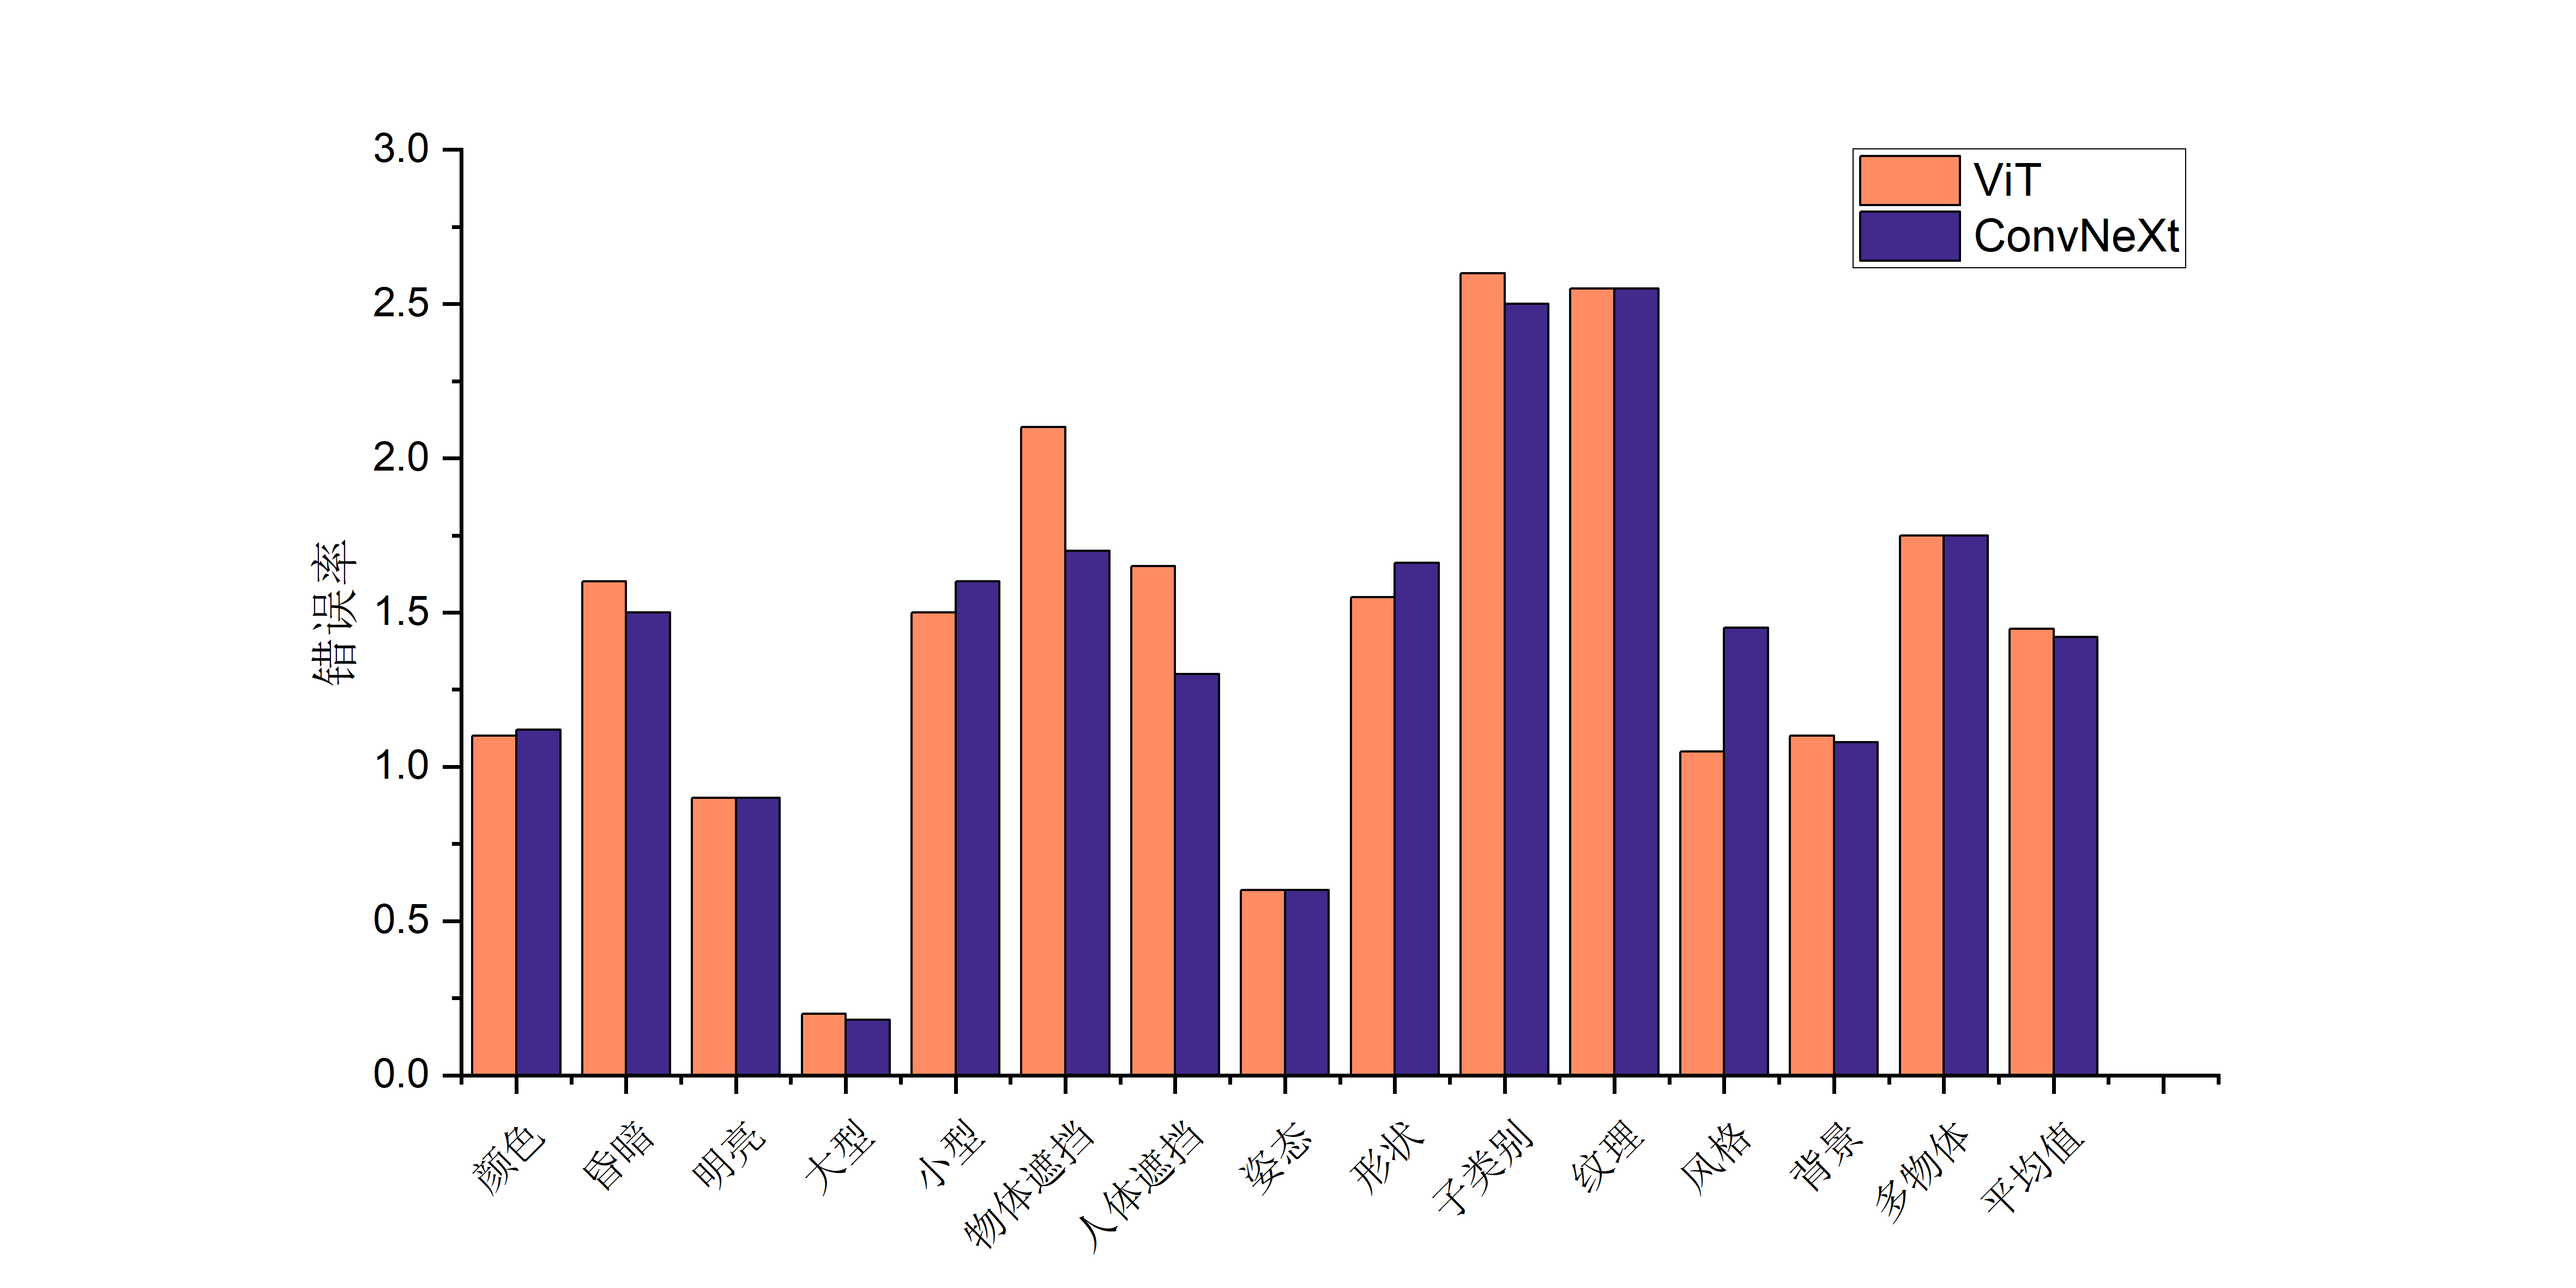
\includegraphics[width=0.9\textwidth]{pics/不同因素.png}
    \caption{ViT和ConvNeXt在不同因素上的错误率}
    \label{fig:error_ratio}
\end{figure}

图\ref{fig:error_ratio}中展示了两种模型对于各种因素的错误率。结果表明两种模型在风格、遮挡、小型物体上的错误率具有较大差异,其中ViT对风格更不敏感,而ConvNeXt对物体尺寸、遮挡更不敏感。此外,两种模型在纹理、子类别、多物体、昏暗环境中都容易犯错误,而在明亮、大型物体、不同姿态的环境中表现良好。

\begin{figure}[H]
    \centering
    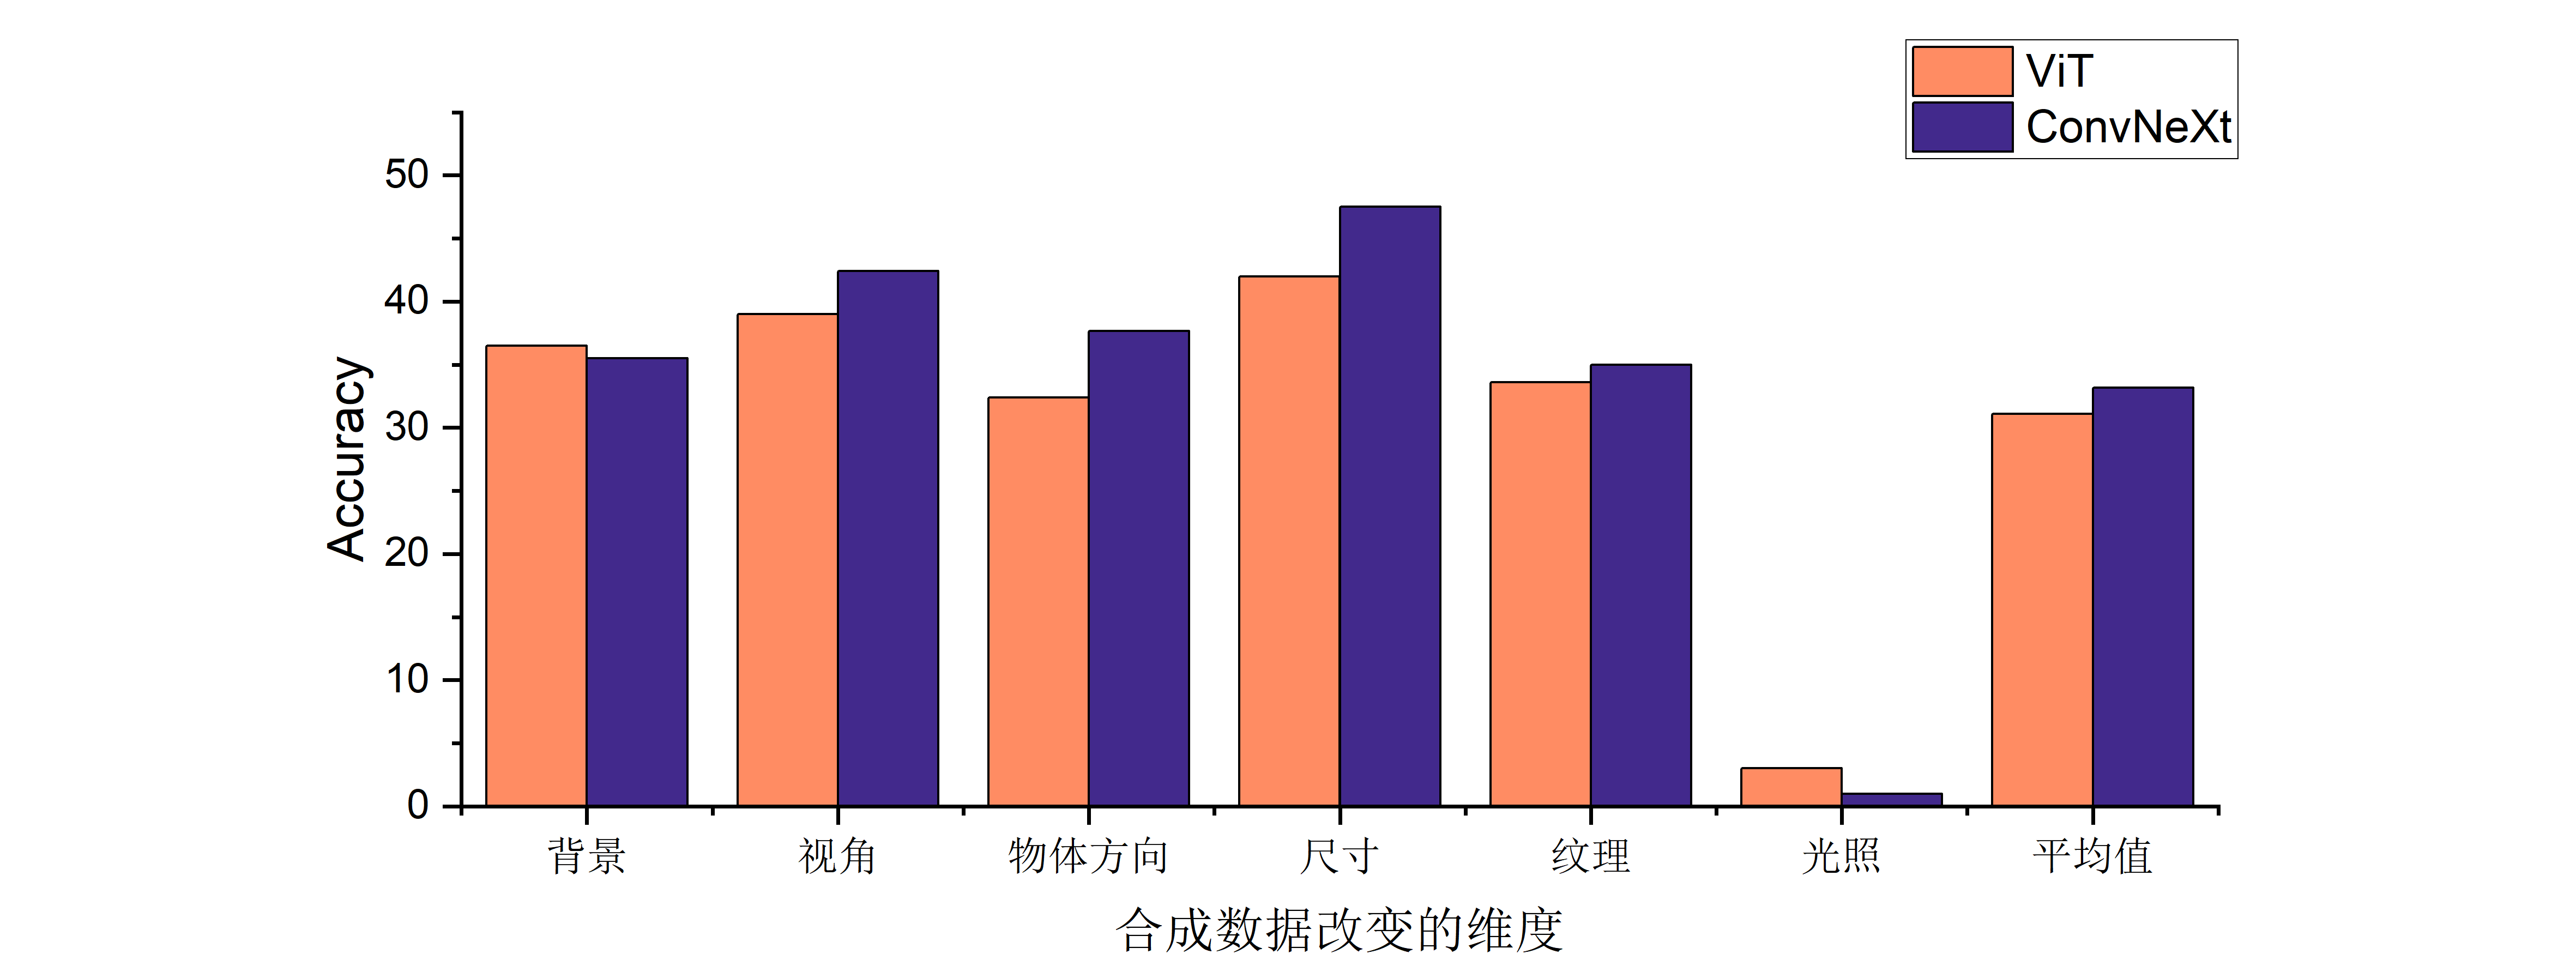
\includegraphics[width=\textwidth]{pics/合成数据.png}
    \caption{合成数据准确性比较}
    \label{fig:synthetic data}
\end{figure}

与人类注释的数据不同,合成数据集允许精确控制相机角度、物体位置和纹理等因素。PUG-ImageNet是一个合成数据集,包含ImageNet类别的照片般逼真的图像并提供属性标签。该图像使用软件引擎生成,允许系统地改变每个对象的姿势、大小、纹理、光线和背景等因素。本文测试了PUG-ImageNet中六个不同因素的Top-1准确性结果,如图\ref{fig:synthetic data}所示,ConvNeXt在视角、物体方向、尺寸、纹理等因素上相比ViT都具备更好的性能,而ViT仅在背景、光照因素上具备优势。这说明CNN学习的特征对于物体形变来说更为有效。

\begin{figure}[H]
    \begin{minipage}[t]{0.33\linewidth}
	\centering
	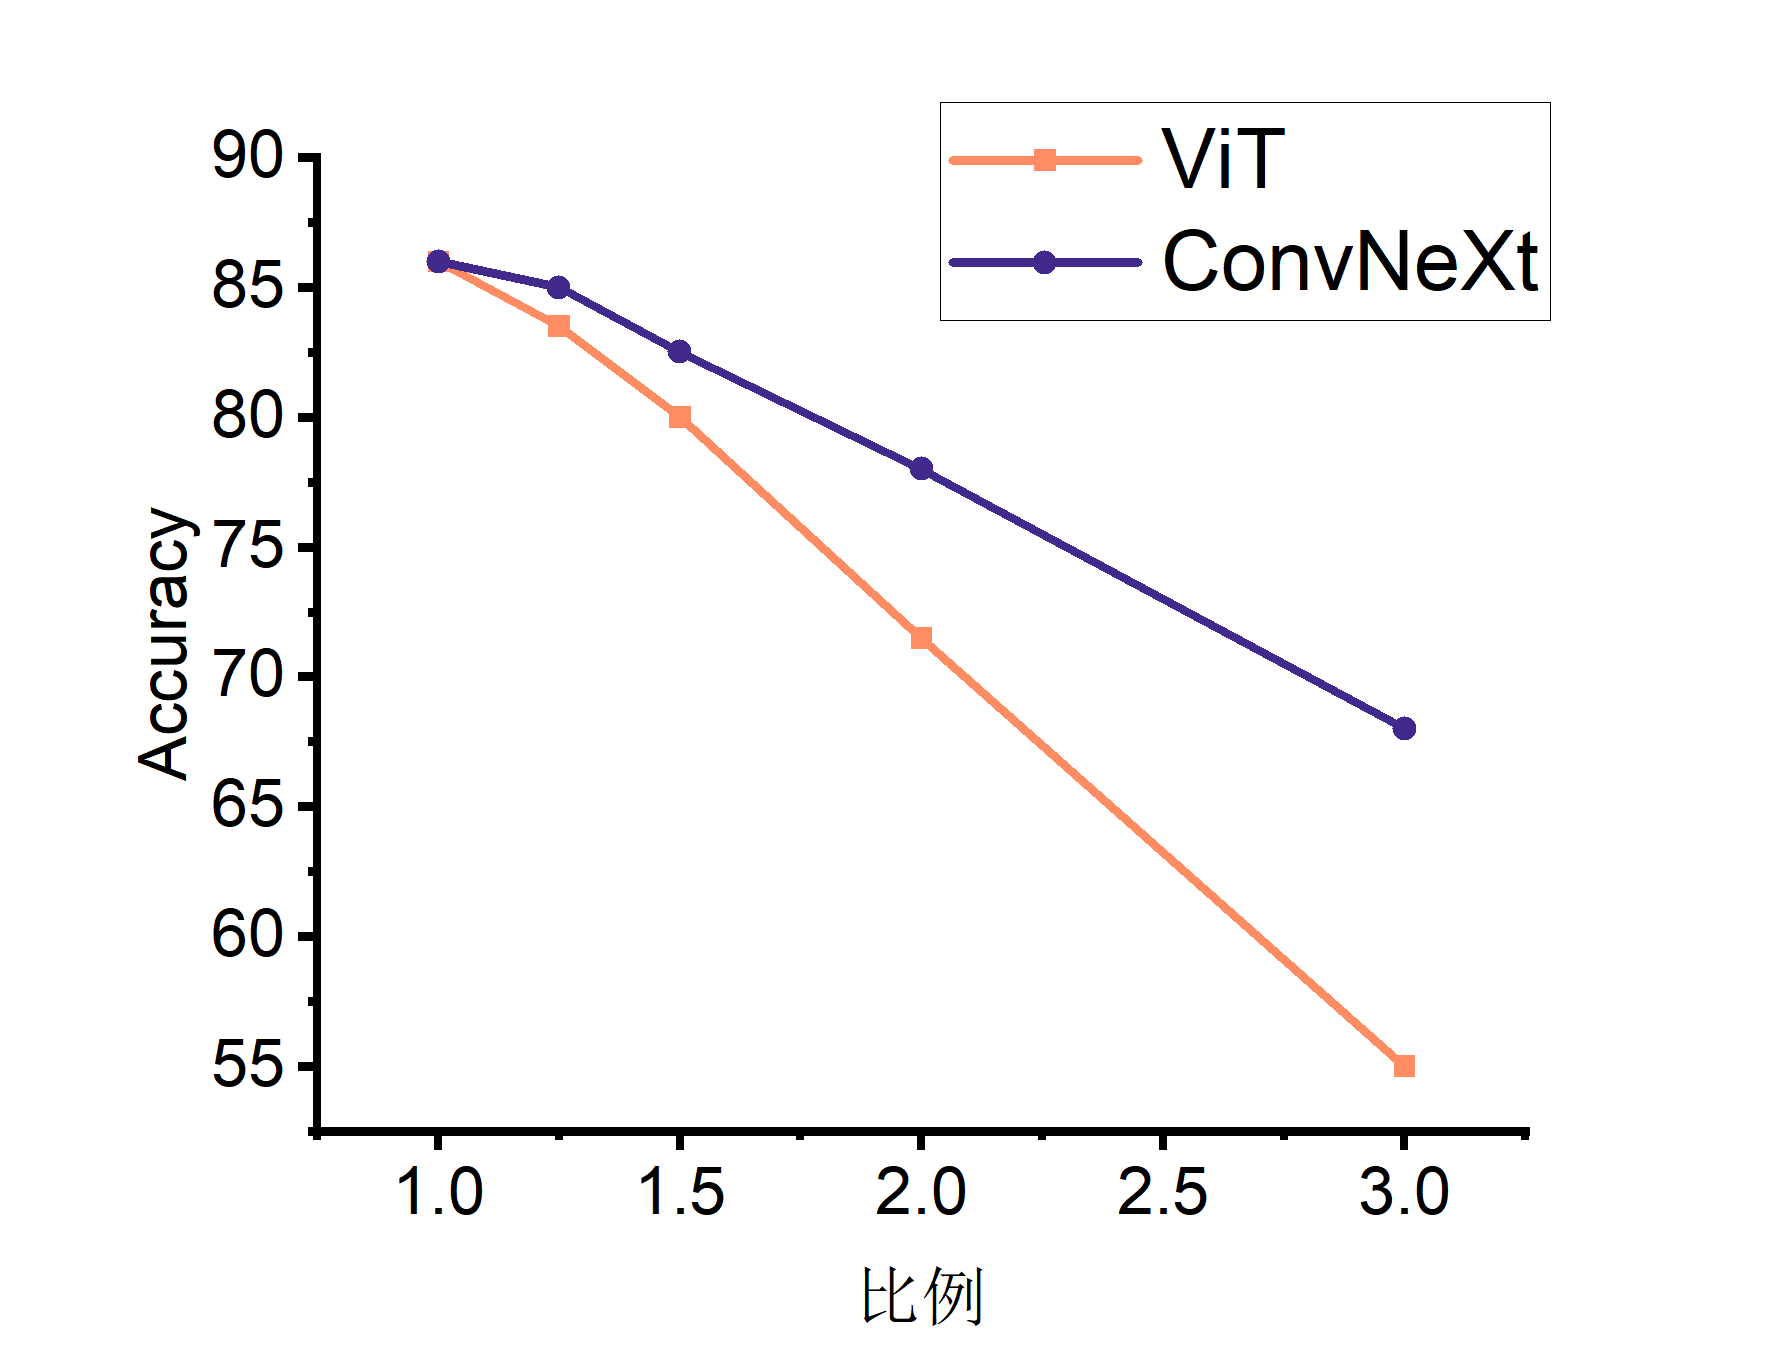
\includegraphics[width=2.2in]{pics/比例.png}
    \end{minipage}
    \begin{minipage}[t]{0.33\linewidth}
	\centering
	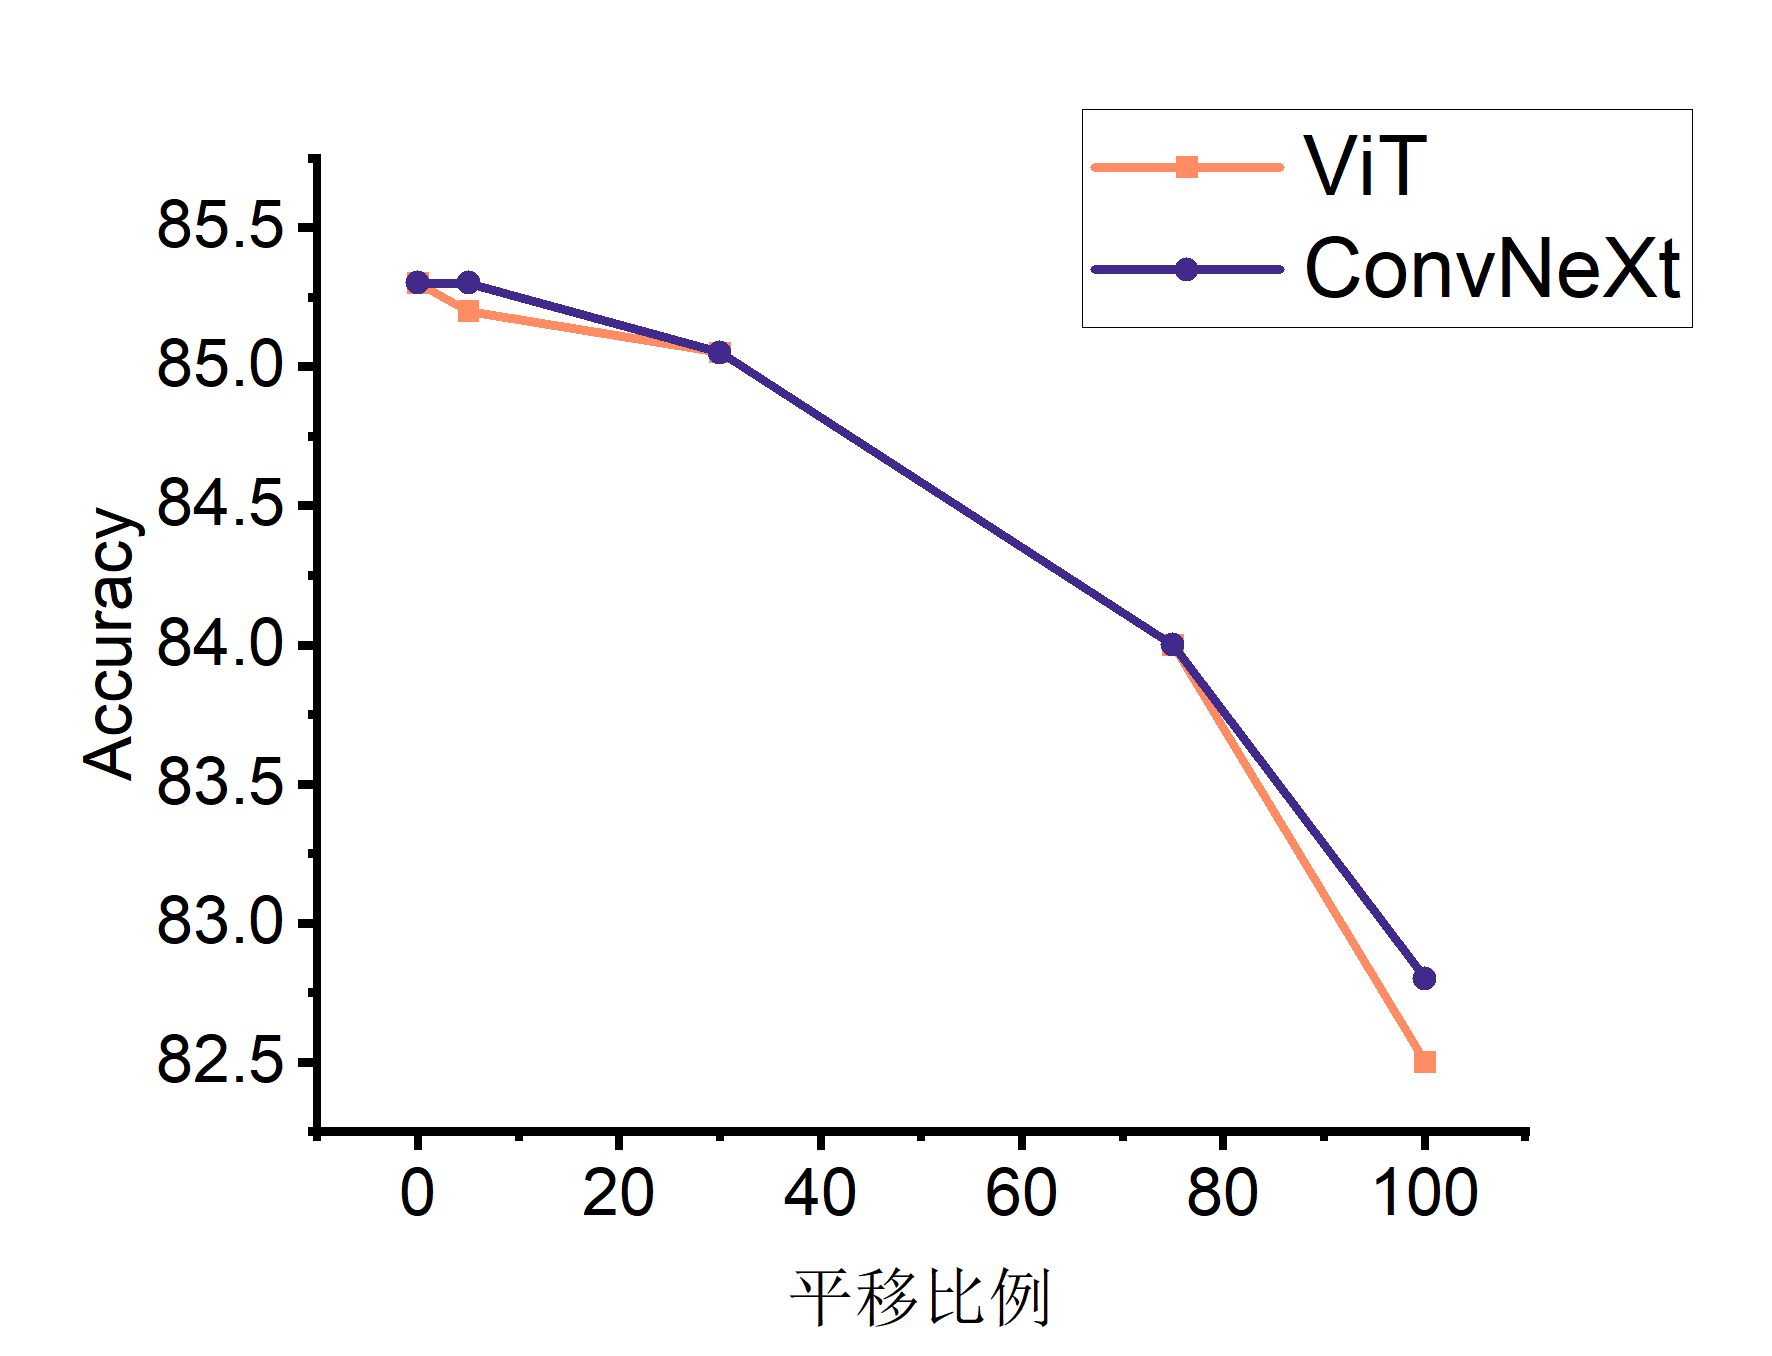
\includegraphics[width=2.2in]{pics/平移比例.png}
    \end{minipage}
    \begin{minipage}[t]{0.33\linewidth}
	\centering
	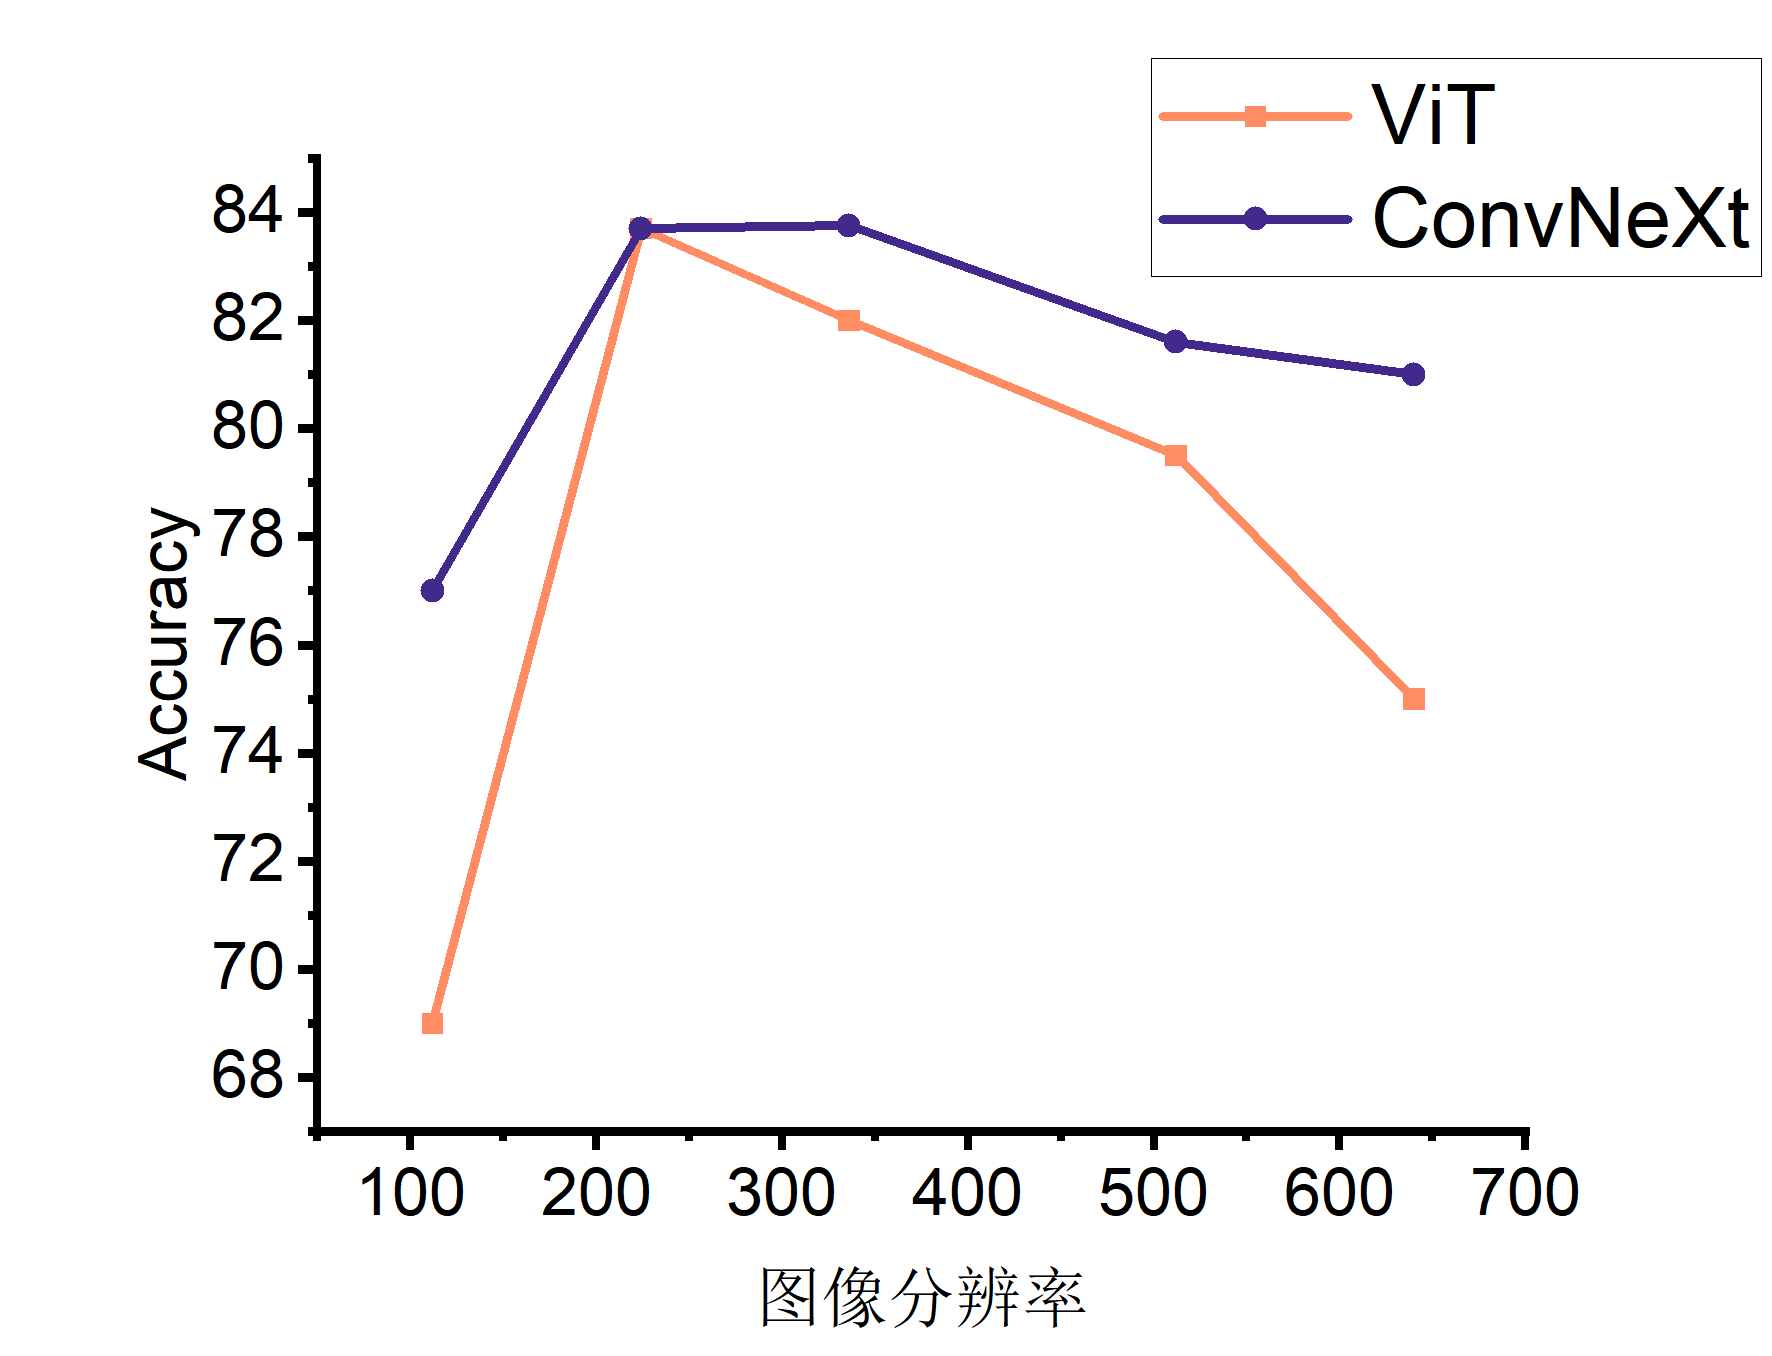
\includegraphics[width=2.2in]{pics/分辨率.png}
    \end{minipage}
    \caption{变换不变性实验结果}
    \label{fig:invariance}
\end{figure}

在实际场景中,数据可能会经过各种各样的变换,如缩放、平移、分辨率改变等,对数据不变具备不变性的模型可以更好应对真实场景的数据变换。以往的实验\cite{azulay2019deep}证明神经网络的性能在简单的输入数据变换下(例如,将图像向左或向上平移几个像素)可能高度不稳定。本文通过对图片进行缩放、平移和分辨率改变对模型的变换不变性进行评估,结果如图\ref{fig:invariance}所示。从图中可以看出,ConvNeXt在不同变换因素下的准确率始终优于ViT。此外,ConvNeXt在图像分辨率变换上的表现稳定,而在缩放、平移变换上出现了较大的性能下降,这说明CNN具备更强大的变换不变性,同时也仍然具备改进空间。

\begin{figure}[H]
    \centering
    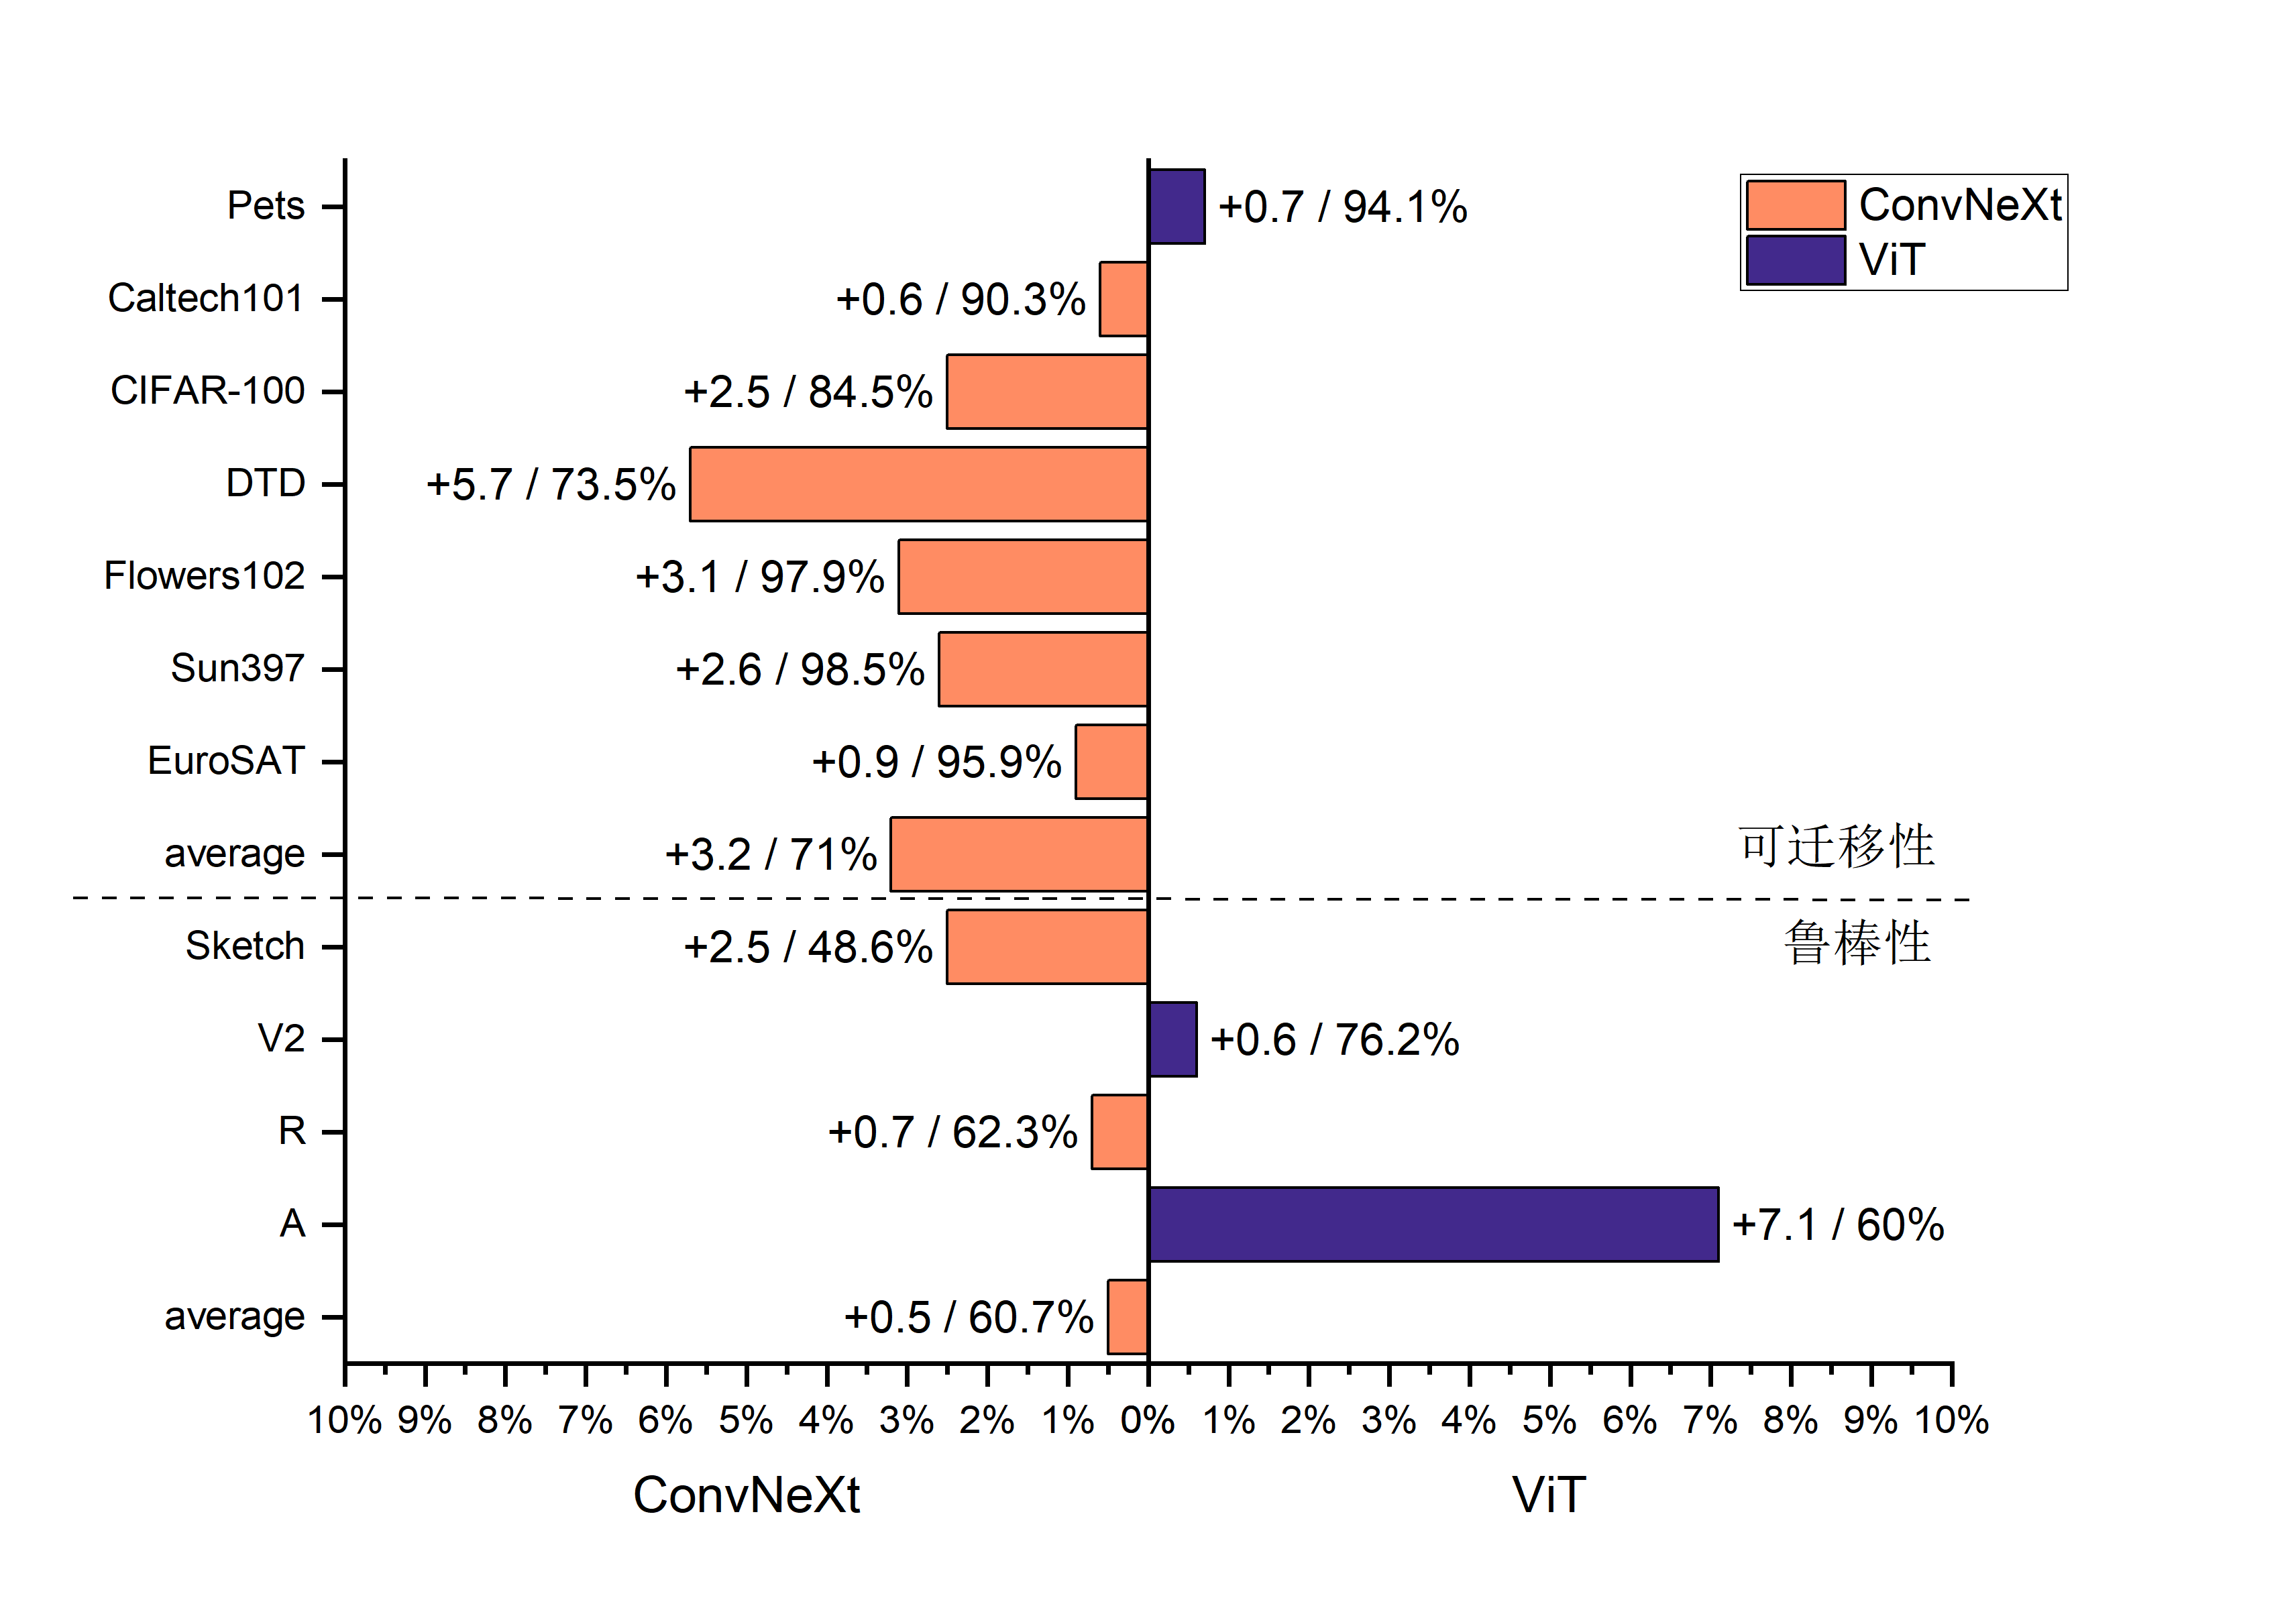
\includegraphics[width=\textwidth]{pics/R&T.2.png}
    \caption{鲁棒性和可迁移性的比较}
    \label{fig:r&t}
\end{figure}

模型性能不仅限于在训练同分布数据集上的准确率,有的模型可能在训练分布的数据上表现出色,但很难将这种表现推广到数据分布的转变。这些转变可以由自然扰动引起,如大气条件(例如,雾、雨),相机噪声或物体位置和方向的变化。模型鲁棒性衡量模型在数据分布变化方面的适应能力,本文在几个包含许多不同类型的自然变化和损坏的数据集测试上评估了模型的鲁棒性,包括ImageNet-V2,ImageNet-A,ImageNet-R,ImageNet-Sketch,这些数据集对ImageNet的图像风格进行处理,包括素描、卡通等不同风格以及对抗性图像,通过对这些图像进行评估,可以反映模型鲁棒性。

模型的迁移学习性能表明其适应新任务的能力,良好的可转移性允许模型使用最小的代价进行快速微调。模型在不显著降低性能的情况下适应这些转变的能力是一种有价值的度量标准,可以衡量其效用和泛化能力。本文使用在ImageNet上预训练的模型,其主要包含自然图像。之后本文采用了7个不同的数据集,分别是EuroSAT,Sun397,Flowers102,DTD,CIFAR-100,Caltech101,Pets,包括如动物、植物、纹理、卫星图像等不同场景。通过对这些数据集进行评估,可以反映模型的泛化能力。

如图\ref{fig:r&t}所示,两种模型在鲁棒性上的表现相似,其中ViT在对抗图像上的表现更好,ConvNeXt则在素描图像上的表现更好,这表明ConvNeXt可能更擅长提取边缘和轮廓信息。此外,ConvNeXt几乎在所有跨数据集任务上的性能更好,这表明CNN的归纳偏置可能是所有数据集之间通用的假设,使得模型具备更为强大的跨数据集迁移学习能力。

\subsection{总结}

% 两者的差异是什么?背后的原因可能是什么?
本章节通过对ViT和ConvNeXt模型的全局和局部特征分析、降维特征分析、性能与泛化能力对比等方面的实验,对两种模型的优劣势进行了详细的分析。通过对两种模型的注意力图、局部特征相似度、层级特征相似度、频域分析、特征图可视化等方面的对比,本文发现ViT模型更倾向于全局特征提取,而ConvNeXt模型更倾向于局部特征提取。通过对两种模型在CIFAR-10和CUB200数据集上的特征可视化和轮廓系数的对比,本文发现ConvNeXt模型在处理细粒度数据集上的性能更优。通过在ImageNet-X和PUG-ImageNet数据集上的性能对比以及变换不变性测试,本文发现ConvNeXt模型对于形状、纹理等因素更不敏感。此外,通过跨域和跨数据集迁移学习实验,本文发现ConvNeXt模型具备更强大的泛化能力。

% 两者的优缺点和适用范围?
综上所述,ViT模型在全局特征提取、对抗性图像学习等方面具备优势。而ConvNeXt模型在局部特征提取、细粒度数据集、跨数据集迁移学习等方面具备优势,此外总体性能也优于ViT。因此,CNN可以更适合于处理细粒度数据集、跨数据集迁移学习、噪声学习等任务,而ViT则更适合于全局特征提取、对抗性图像学习等任务。